\chapter{Ứng dụng của Dữ liệu Thay thế}
\label{ch:M4L3}

% Lesson: Applications of Alternative Data

\section*{Lesson Notes}

MODULE 4 | BÀI 3

\emph{Trong bài học này, chúng ta xem xét các ứng dụng của dữ liệu thay thế (alternative data). Dữ liệu thay thế trong tài chính là những nguồn dữ liệu phi truyền thống được dùng để thu được hiểu biết về xu hướng thị trường, định giá tài sản và các quyết định đầu tư. Điều này đối lập với dữ liệu truyền thống như báo cáo tài chính, hồ sơ công bố của công ty và giá thị trường. Dữ liệu văn bản từ mạng xã hội thuộc nhóm này vì nó phản ánh cảm xúc của công chúng, các bàn tán trên thị trường và sự lan truyền tin tức, những yếu tố có thể ảnh hưởng đến giá tài sản. Cụ thể, dữ liệu Twitter và StockTwits được xem là những nguồn dữ liệu thay thế có giá trị trong kỹ thuật tài chính nhờ tính thời gian thực và trọng tâm vào các thảo luận tài chính và hoạt động của thị trường chứng khoán.}

\begin{lstlisting}[language=Python,escapeinside={(*@}{@*)}]
# (*@Tải@*) (*@các@*) (*@thư@*) (*@viện@*)
import datetime
import matplotlib.pyplot as plt
import os
import pandas as pd
import plotly.express as px
import re
import requests
import zipfile

from datetime import datetime, timedelta
\end{lstlisting}

\section{Dữ liệu Twitter là gì}

Dữ liệu Twitter là lượng thông tin khổng lồ được tạo ra và chia sẻ trên nền tảng Twitter. Đây là một tập hợp thông tin đồ sộ do người dùng tạo ra trên nền tảng, bao gồm tweet, hồ sơ cá nhân, tin nhắn, xu hướng, phương tiện đa truyền thông và các tương tác. Dữ liệu này chủ yếu có sẵn ở định dạng JSON thông qua Twitter API, dù các phương pháp khác như thu thập dữ liệu web (web scraping) và công cụ của bên thứ ba cũng có thể được sử dụng. Việc truy cập dữ liệu lịch sử thường bị hạn chế, và Academic Research Track (Chương trình Nghiên cứu Học thuật) mang lại quyền truy cập rộng hơn cho các nhà nghiên cứu. Dữ liệu Twitter là nguồn tài nguyên phong phú để hiểu và phân tích thế giới trực tuyến. Dữ liệu này có giá trị đối với phân tích mạng xã hội, nghiên cứu thị trường, tình báo kinh doanh, tin tức, y tế công cộng, khoa học chính trị và nghiên cứu học thuật, cho phép thu được hiểu biết về hành vi người dùng, dư luận và các sự kiện thời gian thực.

Cấu trúc và định dạng dữ liệu:

\begin{itemize}
  \item JSON: Twitter API chủ yếu cung cấp dữ liệu ở định dạng JSON (JavaScript Object Notation). JSON là một định dạng trao đổi dữ liệu gọn nhẹ, dễ đọc và dễ viết đối với con người, đồng thời dễ phân tích cú pháp và tạo ra đối với máy. Mỗi tweet, hồ sơ người dùng hoặc đối tượng dữ liệu khác được biểu diễn như một đối tượng JSON với nhiều thuộc tính và giá trị.
  \item CSV/TSV: Dữ liệu Twitter cũng có thể được xuất hoặc chuyển đổi sang định dạng CSV (Comma-Separated Values) hoặc TSV (Tab-Separated Values) để phân tích trong phần mềm bảng tính hoặc các công cụ khác.
  \item Cơ sở dữ liệu: Đối với phân tích và lưu trữ quy mô lớn, dữ liệu Twitter thường được nạp vào các cơ sở dữ liệu như MySQL, PostgreSQL hoặc các cơ sở dữ liệu NoSQL như MongoDB.
\end{itemize}

Truy cập dữ liệu Twitter và các hạn chế:

\begin{itemize}
  \item Twitter API: Dù Twitter API là cách truy cập dữ liệu mạnh mẽ, vẫn có những giới hạn và hạn chế. Chúng bao gồm giới hạn tần suất (rate limit) về số yêu cầu có thể gửi, chỉ truy cập được một phần dữ liệu lịch sử (thường là 7 ngày gần nhất đối với API tiêu chuẩn), và yêu cầu về tài khoản nhà phát triển cùng khóa API.
  \item Academic Research Track: Đối với các nhà nghiên cứu học thuật, Twitter cung cấp ``Academic Research Track'' với mức truy cập nâng cao và lượng dữ liệu sẵn có lớn hơn. Chương trình này đòi hỏi một đề xuất nghiên cứu chi tiết và quy trình phê duyệt.
  \item Thiên lệch dữ liệu và các cân nhắc đạo đức: Cần lưu ý những thiên lệch tiềm ẩn trong dữ liệu Twitter, chẳng hạn việc một số nhóm nhân khẩu học hoặc quan điểm được đại diện quá mức. Các cân nhắc đạo đức là thiết yếu, bao gồm tôn trọng quyền riêng tư của người dùng, xin sự đồng ý có hiểu biết khi cần thiết và tránh lan truyền thông tin sai lệch. Dữ liệu Twitter vốn thiên về những người dùng tích cực và các ý kiến được chia sẻ công khai. Tập dữ liệu này có thể không đại diện cho quan điểm của toàn bộ cộng đồng nhà đầu tư.
  \item Tính thưa thớt và chất lượng dữ liệu: Tập dữ liệu có thể chứa những khoảng trống hoặc những giai đoạn có khối lượng tweet thấp, điều này có thể ảnh hưởng đến phân tích. Điều thiết yếu là kiểm tra chất lượng dữ liệu và xử lý mọi vấn đề tiềm ẩn như giá trị thiếu hoặc sự không nhất quán trước khi tiến hành phân tích.
\end{itemize}

Có nhiều lựa chọn để tải các tập dữ liệu Twitter có sẵn, với nhiều con đường phục vụ cả nhà nghiên cứu lẫn người dùng thông thường, với các mức truy cập và đặc thù dữ liệu khác nhau:

\begin{itemize}
  \item Dành cho nhà nghiên cứu: Twitter Academic Research Track cung cấp quyền truy cập toàn diện nhất, nhưng đòi hỏi nộp đơn và được phê duyệt.
  \item Các lựa chọn công khai: Các nền tảng như Kaggle, figshare, Zenodo, Data.World, Hugging Face, IEEE DataPort và Mendeley Data lưu trữ nhiều tập dữ liệu về các chủ đề khác nhau, sẵn sàng để tải xuống. Kaggle là nền tảng do cộng đồng vận hành nổi bật nhất trong số được nêu. IEEE DataPort tập trung hơn vào việc chia sẻ dữ liệu nghiên cứu trong các lĩnh vực cụ thể. Hugging Face là nền tảng do cộng đồng dẫn dắt, chuyên về NLP và các lĩnh vực liên quan.
  \item Các nguồn chuyên biệt: Các cơ quan chính phủ và tổ chức có thể cung cấp các tập dữ liệu liên quan đến những sự kiện hoặc chủ đề cụ thể.
\end{itemize}

Khi sử dụng các nền tảng này, có lẽ điều quan trọng nhất là tuân thủ các thực hành dữ liệu có trách nhiệm và ưu tiên tính hợp pháp, sự bảo vệ người dùng và ứng xử có đạo đức, nhằm bảo đảm niềm tin và tác động xã hội tích cực. Cấp phép dữ liệu, quyền riêng tư của người dùng và các cân nhắc đạo đức là thiết yếu cho việc sử dụng dữ liệu có trách nhiệm. Việc cấp phép bảo đảm tuân thủ pháp lý, quyền riêng tư bảo vệ thông tin cá nhân, và đạo đức định hướng các thực hành dữ liệu công bằng và tôn trọng. Những khía cạnh này cũng có vai trò then chốt đối với dữ liệu công khai, đòi hỏi tuân thủ các điều khoản giấy phép, ẩn danh hóa để bảo vệ quyền riêng tư và ý thức về những thiên lệch tiềm ẩn để phân tích có đạo đức.

\subsection{Lấy dữ liệu Twitter}

Trong bài học này, chúng ta khám phá dữ liệu Stock Market Tweets từ IEEE Dataport, có tại \url{https://dx.doi.org/10.21227/g8vy-5w61}. IEEE DataPort là một kho lưu trữ được tuyển chọn dành cho dữ liệu nghiên cứu, chủ yếu tập trung vào các lĩnh vực kỹ thuật và công nghệ. Kho này do Viện Kỹ sư Điện và Điện tử (Institute of Electrical and Electronics Engineers, IEEE) vận hành và khuyến khích các nhà nghiên cứu chia sẻ tập dữ liệu của mình để thúc đẩy tri thức trong lĩnh vực tương ứng. Tập dữ liệu này chứa một bộ sưu tập các tweet liên quan đến thị trường chứng khoán, đặc biệt tập trung vào chỉ số S\&P 500. Mục tiêu là cung cấp dữ liệu cho các nhà nghiên cứu và người thực hành quan tâm đến việc phân tích mối quan hệ giữa cảm xúc trên mạng xã hội và biến động của thị trường chứng khoán.

Tập dữ liệu này được cung cấp theo giấy phép Creative Commons Attribution 4.0 International (CC BY 4.0). Giấy phép này cho phép sử dụng, chia sẻ, chỉnh sửa và phân phối lại dữ liệu một cách tự do, miễn là ghi công phù hợp cho những người tạo ra bản gốc.

Tập dữ liệu bao phủ các tweet từ ngày 9 tháng 4 năm 2020 đến ngày 16 tháng 7 năm 2020. Khoảng thời gian này cung cấp lượng dữ liệu đáng kể cho phân tích và bao quát nhiều điều kiện thị trường khác nhau. Dữ liệu được thu thập bằng thẻ S\&P 500 (\#SPX500), các đề cập đến 25 công ty hàng đầu trong chỉ số S\&P 500, và thẻ Bloomberg (\#stocks). Dữ liệu được đóng gói trong một tệp lưu trữ ZIP gồm hai tệp CSV: tệp 'tweets\_labelled\_09042020\_16072020.csv' gồm 5.000 tweet được chọn bằng lấy mẫu ngẫu nhiên. Trong số 5.000 tweet đó, 1.300 tweet được gán nhãn thủ công vào các lớp tích cực, trung lập hoặc tiêu cực. Tệp thứ hai 'tweets\_remaining\_09042020\_16072020.csv' chứa phần còn lại của các tweet.

Đoạn mã dưới đây được thiết kế để giải nén một tệp ZIP chứa dữ liệu Twitter, rồi định vị tất cả các tệp CSV trong thư mục đã giải nén để xử lý tiếp. Mã lặp qua danh sách các tệp CSV chứa dữ liệu Twitter, đọc từng tệp vào một DataFrame pandas, chuẩn hóa tên cột chứa văn bản tweet, rồi gộp tất cả các DataFrame thành một DataFrame duy nhất có tên \texttt{twitter\_df}:

\begin{lstlisting}[language=Python,escapeinside={(*@}{@*)}]
# (*@Giải@*) (*@nén@*) (*@tệp@*) ZIP (*@vào@*) (*@thư@*) (*@mục@*) (*@có@*) (*@tên@*) 'extracted_tweets'
with zipfile.ZipFile('tweets.zip', 'r') as zip_ref:
    zip_ref.extractall('extracted_tweets')

# (*@Lấy@*) danh (*@sách@*) (*@các@*) (*@tệp@*) CSV trong (*@thư@*) (*@mục@*) 'tweets' (*@bên@*) trong
tweets_folder = 'extracted_tweets/tweets'
csv_files = [f for f in os.listdir(tweets_folder) if f.endswith('.csv')]

# (*@Lặp@*) qua (*@các@*) (*@tệp@*) CSV (*@và@*) (*@đọc@*) (*@chúng@*) (*@vào@*) (*@các@*) DataFrame
dfs = []
for csv_file in csv_files:
    file_path = os.path.join(tweets_folder, csv_file)
    df = pd.read_csv(file_path, sep=';')

    # (*@Đổi@*) (*@tên@*) (*@cột@*) 'full_text' (*@hoặc@*) 'text' (*@thành@*) (*@tên@*) chung 'tweet_text'
    if 'full_text' in df.columns:
        df = df.rename(columns={'full_text': 'tweet_text'})
    elif 'text' in df.columns:
        df = df.rename(columns={'text': 'tweet_text'})

    dfs.append(df)

# (*@Nối@*) (*@tất@*) (*@cả@*) (*@các@*) DataFrame (*@thành@*) (*@một@*) DataFrame duy (*@nhất@*) (*@và@*) (*@hiển@*) (*@thị@*) (*@nó@*)
twitter_df = pd.concat(dfs, ignore_index=True)
twitter_df
\end{lstlisting}

\begin{lstlisting}[escapeinside={(*@}{@*)}]
BadZipFile
\end{lstlisting}

\subsection{Điều chỉnh múi giờ trong dữ liệu Twitter}

Bây giờ hãy quan sát định dạng ngày và giờ trong cột 'created\_at'. Ký hiệu ``+00:00'' trong các giá trị của 'created\_at' chỉ một múi giờ. Nó biểu diễn độ lệch so với Giờ Phối hợp Quốc tế (UTC), trong trường hợp này là 0 giờ. Điều này có nghĩa là các dấu thời gian đang ở chính UTC. Hãy chuyển đổi chúng sang múi giờ New York. Ta thực hiện bằng hàm \texttt{pd.to\_datetime()}, hàm này chuyển cột 'created\_at' thành các đối tượng DateTime của pandas. Sau đó ta áp dụng chuỗi hàm \texttt{.dt.tz\_convert('America/New\_York')}, hàm này chuyển các đối tượng DateTime sang múi giờ New York bằng tên múi giờ IANA 'America/New\_York'. Điều này bảo đảm các dấu thời gian được điều chỉnh theo các lần chuyển đổi giờ mùa hè tại New York:

\begin{lstlisting}[language=Python,escapeinside={(*@}{@*)}]
# (*@Chuyển@*) (*@các@*) (*@dấu@*) (*@thời@*) gian sang (*@múi@*) (*@giờ@*) New York
twitter_df['created_at'] = pd.to_datetime(twitter_df['created_at']).dt.tz_convert('America/New_York')
twitter_df
\end{lstlisting}

\begin{lstlisting}[escapeinside={(*@}{@*)}]
NameError
\end{lstlisting}

\subsection{Phát hiện retweet trong dữ liệu Twitter}

Trên Twitter, ``RT'' là chữ viết tắt phổ biến của ``retweet''. Khi một người dùng muốn chia sẻ tweet của người khác với những người theo dõi của mình, họ có thể retweet. ``RT'' là dấu hiệu then chốt của các retweet trên Twitter. Nó được dùng trong các retweet thủ công, retweet có trích dẫn, và là một quy ước đã trở thành một phần của văn hóa Twitter. Bằng cách tìm kiếm ``RT'' ở đầu các tweet, chúng ta có thể nhận diện retweet một cách hiệu quả trong phân tích dữ liệu.

Bây giờ hãy lấy bộ sưu tập tweet của chúng ta và tách chúng thành hai nhóm: một nhóm cho retweet và một nhóm cho tweet gốc (hoặc các loại tweet khác không phải retweet). Đoạn mã dưới đây lấy DataFrame \texttt{twitter\_df} chứa dữ liệu Twitter và tách nó thành hai DataFrame mới bằng cách lọc cột 'tweet\_text'. Sau đó mã hiển thị cả \texttt{retweets\_df} và \texttt{remainder\_df} bằng hàm \texttt{display()}:

\begin{lstlisting}[language=Python,escapeinside={(*@}{@*)}]
# (*@Tạo@*) (*@một@*) DataFrame (*@chỉ@*) (*@chứa@*) (*@các@*) retweet
retweets_df = twitter_df[twitter_df['tweet_text'].str.startswith('RT')]

# (*@Tạo@*) (*@một@*) DataFrame (*@chứa@*) (*@các@*) tweet (*@không@*) (*@phải@*) retweet
remainder_df = twitter_df[~twitter_df['tweet_text'].str.startswith('RT')]

# (*@Hiển@*) (*@thị@*) (*@các@*) DataFrame
print("## Retweets DataFrame:")
print("This DataFrame contains only retweets from the Twitter data.")
display(retweets_df)

print("\n## Remainder DataFrame:")
print("This DataFrame contains tweets that are not retweets.")
display(remainder_df)
\end{lstlisting}

\begin{lstlisting}[escapeinside={(*@}{@*)}]
NameError
\end{lstlisting}

Ở đây ta thấy \texttt{retweets\_df} có 350.752 hàng và \texttt{remainder\_df} có 577.921 hàng. Cần lưu ý rằng các DataFrame được tách dựa trên việc một tweet có phải là retweet hay không. Số hàng của \texttt{retweets\_df} và \texttt{remainder\_df} cho ta ý niệm về tỷ lệ retweet trong tập dữ liệu, nhưng điều này không cho biết trực tiếp có bao nhiêu tweet gốc riêng biệt đã được retweet. Một tweet gốc có thể được nhiều người dùng khác nhau retweet nhiều lần, vì vậy 350.752 hàng trong \texttt{retweets\_df} có thể đại diện cho một số lượng tweet gốc riêng biệt nhỏ hơn nhiều đã được retweet nhiều lần. Chúng ta cũng nên xét đến hiệu ứng độ trễ thời gian dựa trên hành vi Twitter điển hình. Rất có khả năng phần lớn các retweet trong tập dữ liệu của chúng ta thuộc cùng giai đoạn, nhưng một số retweet sẽ đến từ giai đoạn sớm hơn đôi chút so với các tweet gốc mà chúng ta đã thu thập.

\subsection{Tìm hiểu phân phối của các tweet}

Bây giờ hãy thử tìm hiểu phân phối của các tweet theo thời gian. Đoạn mã dưới đây lấy cột 'created\_at' làm chỉ mục để lấy mẫu lại (resampling). Sau đó nó lấy mẫu lại dữ liệu theo tuần và tính số lượng tweet trong mỗi khoảng tuần. Cuối cùng, nó đếm số tweet xảy ra trong mỗi tuần:

\begin{lstlisting}[language=Python,escapeinside={(*@}{@*)}]
# (*@Lấy@*) (*@số@*) (*@lượng@*) tweet theo (*@tuần@*)
weekly_counts = twitter_df.set_index('created_at').resample('W-MON', label='left', closed='left').count()
weekly_counts = weekly_counts.rename_axis(index="Week Starting")
display(weekly_counts)
\end{lstlisting}

\begin{lstlisting}[escapeinside={(*@}{@*)}]
NameError
\end{lstlisting}

Ở đây \texttt{.resample('W-MON', label='left', closed='left')} là phần cốt lõi của thao tác. \texttt{.resample('W-MON')} lấy mẫu lại dữ liệu vào các khoảng theo tuần, bắt đầu từ thứ Hai ('W-MON'). \texttt{label='left'} chỉ ra rằng nhãn của mỗi khoảng phải là mép trái (điểm bắt đầu) của khoảng. \texttt{closed='left'} quy định mép trái của mỗi khoảng là đóng (được bao gồm trong khoảng). Điều này có nghĩa là các tweet được tạo vào thứ Hai sẽ được tính vào khoảng của tuần đó.

Bảng phân phối theo tuần này tạo cơ hội quan sát các xu hướng hoạt động tweet theo thời gian. Ở đây ta thấy số lượng tweet nhìn chung dao động nhưng có vẻ tương đối cao trong suốt tháng Sáu và tháng Bảy. Và có hai tuần (11 tháng 5 và 18 tháng 5) không ghi nhận tweet nào, và có thể cả tuần kế tiếp (25 tháng 5) cũng có hoạt động tweet giảm. Điều này có thể cho thấy một vấn đề trong thu thập dữ liệu hoặc một giai đoạn hoạt động thấp.

\subsection{Trực quan hóa dữ liệu Twitter}

Bằng cách xem xét khối lượng dữ liệu và áp dụng các kỹ thuật trực quan hóa phù hợp, chúng ta có thể thu được những hiểu biết có ý nghĩa hơn từ biểu đồ số lượng tweet hàng ngày. Bây giờ hãy nhóm dữ liệu theo ngày và vẽ số lượng tweet hàng ngày cho DataFrame \texttt{twitter\_df} để khảo sát. Đoạn mã dưới đây trước hết nhóm DataFrame \texttt{twitter\_df} theo phần ngày của cột 'created\_at' bằng \texttt{dt.date} để trích xuất ngày. Việc này tạo ra các nhóm tweet cho mỗi ngày. Sau đó nó đếm số tweet trong mỗi nhóm bằng \texttt{['tweet\_text'].count()}, hàm đếm các giá trị không rỗng trong cột 'tweet\_text'. Tiếp theo chúng ta vẽ dữ liệu:

\begin{lstlisting}[language=Python,escapeinside={(*@}{@*)}]
# (*@Nhóm@*) theo (*@ngày@*) (*@và@*) (*@đếm@*)
daily_tweet_counts_twitter_all = twitter_df.groupby(twitter_df['created_at'].dt.date)['tweet_text'].count()

# (*@Vẽ@*) (*@biểu@*) (*@đồ@*)
plt.figure(figsize=(12, 6))

plt.plot(daily_tweet_counts_twitter_all.index, daily_tweet_counts_twitter_all.values, label='Twitter (All Data)', marker='o')

plt.xlabel('Date')
plt.ylabel('Number of Tweets')
plt.title('Daily Tweet Counts - Twitter (All Data)')
plt.legend()
plt.grid(True)

plt.xticks(rotation=45, ha='right')  # Xoay (*@nhãn@*) (*@trục@*) x (*@để@*) (*@dễ@*) (*@đọc@*) (*@hơn@*)

plt.tight_layout()  # (*@Điều@*) (*@chỉnh@*) (*@bố@*) (*@cục@*) (*@để@*) (*@tránh@*) (*@nhãn@*) (*@chồng@*) (*@lên@*) nhau
plt.show()
\end{lstlisting}

\begin{lstlisting}[escapeinside={(*@}{@*)}]
NameError
\end{lstlisting}

Bằng cách xem xét biểu đồ, chúng ta có thể nhận diện mọi khoảng trống hoặc giai đoạn có số lượng tweet thấp hơn đáng kể hoặc bằng không. Những khoảng trống này có thể cho thấy dữ liệu bị thiếu hoặc những giai đoạn hoạt động tweet suy giảm. Nếu cần khảo sát sâu hơn các khoảng trống hoặc mẫu hình cụ thể, chúng ta có thể điều chỉnh khoảng thời gian của biểu đồ hoặc thêm chú thích để làm nổi bật các vùng đáng quan tâm. Trong trường hợp của chúng ta, ta biết rằng có một khoảng trống trong giai đoạn từ ngày 10 tháng 5 đến ngày 27 tháng 5 năm 2020. Điều này có nghĩa là hoặc không có tweet nào được thu thập hay ghi nhận trong giai đoạn đó, hoặc chúng đã bị lọc bỏ trong quá trình xử lý dữ liệu.

Có nhiều kỹ thuật điền khuyết dữ liệu (data imputation) để lấp đầy dữ liệu bị thiếu. Với cách tiếp cận đơn giản, chúng ta có thể lấp khoảng trống bằng số lượng tweet trung bình của những ngày trước và sau khoảng trống. Với những tình huống phức tạp hơn, chúng ta có thể khám phá các kỹ thuật điền khuyết chuỗi thời gian hoặc các mô hình học máy để dự đoán các giá trị bị thiếu dựa trên các mẫu hình trong dữ liệu hiện có. Tuy nhiên, việc này cần được thực hiện thận trọng và có ý thức về những thiên lệch tiềm ẩn do điền khuyết đưa vào. Trong trường hợp của chúng ta, không kỹ thuật nào trong số này có thể chính xác, vì có một khoảng trống đáng kể mà trong đó các xu hướng hoặc sự kiện có thể rất khó lường để suy ra hay mô hình hóa. Do đó, chúng ta tạm giữ nguyên khoảng trống này và tiếp tục các khám phá sâu hơn.

\subsection{Phát hiện cashtag và hashtag trong dữ liệu Twitter}

Trong các tweet Twitter, mã cổ phiếu có thể xuất hiện dưới dạng cashtag (ví dụ \$AAPL, \$GOOG) hoặc hashtag (ví dụ \#AAPL, \#GOOG), cả hai thường đại diện cho mã chứng khoán (ticker) của một công ty. Cashtag ngày càng phổ biến, nhưng hashtag vẫn được dùng cho các thảo luận hoặc sự kiện liên quan đến cổ phiếu ở phạm vi rộng hơn. Các ký hiệu này có thể được đặt ở bất kỳ vị trí nào trong một tweet và thường cung cấp ngữ cảnh cho thông điệp, gắn nó với một cổ phiếu hoặc chủ đề cụ thể.

Bây giờ hãy khám phá vài hiểu biết về việc những cổ phiếu nào được thảo luận thường xuyên nhất trong dữ liệu Twitter của chúng ta. Đoạn mã dưới đây trước hết trích xuất các mã cổ phiếu từ phần đầu của mỗi tweet trong DataFrame \texttt{twitter\_df} bằng biểu thức chính quy (regular expression) và lưu chúng vào một cột mới 'stock\_symbols'. Sau đó, nó ``bung'' (explode) cột này để tạo các hàng riêng cho mỗi mã trong một tweet. Nó chuyển các mã sang chữ thường, đếm số lần xuất hiện, sắp xếp theo tần suất giảm dần, và cuối cùng hiển thị 10 mã cổ phiếu được đề cập thường xuyên nhất trong tập dữ liệu:

\begin{lstlisting}[language=Python,escapeinside={(*@}{@*)}]
# (*@Phát@*) (*@hiện@*) (*@mã@*) (*@cổ@*) (*@phiếu@*) (*@và@*) hashtag
twitter_df['cashtags_hashtags'] = twitter_df['tweet_text'].str.findall(r'(?:\$|#)([a-zA-Z]+\.*[a-zA-Z]+)')
twitter_df.explode('cashtags_hashtags')['cashtags_hashtags'].str.lower().value_counts().sort_values(ascending=False).head(10)
\end{lstlisting}

\begin{lstlisting}[escapeinside={(*@}{@*)}]
cashtags_hashtags
stocks         262381
spx            190857
aapl           123629
spy            115031
amzn           108484
fb              85685
es              66068
stockmarket     65091
msft            62018
trading         60261
Name: count, dtype: int64
\end{lstlisting}

Ở đây \texttt{.str.findall(r'(?:\textbackslash{}\$|\#)([a-zA-Z]+\textbackslash{}.*[a-zA-Z]+)')} áp dụng một biểu thức chính quy để tìm và trích xuất cashtag và hashtag từ văn bản tweet. Hãy phân tích biểu thức chính quy này:

\begin{itemize}
  \item \texttt{(?: ... )}: Tạo một nhóm không bắt (non-capturing group). Điều này có nghĩa là phần này của biểu thức chính quy được dùng để khớp, nhưng nội dung khớp sẽ không được bắt và lưu riêng.
  \item \texttt{\textbackslash{}\$|\#}: Khớp với một dấu đô la nguyên văn (\$) hoặc một dấu thăng hashtag (\#). Ký hiệu \texttt{ | } biểu diễn điều kiện ``hoặc''.
  \item \texttt{[a-zA-Z]+}: Khớp với một hoặc nhiều chữ cái (a-z, A-Z).
  \item \texttt{\textbackslash{}.*}: Khớp với không hoặc một dấu chấm (.), cho phép các mã có dấu chấm (ví dụ \$BRK.B).
  \item \texttt{[a-zA-Z]+}: Lại khớp với một hoặc nhiều chữ cái, bắt phần còn lại của mã sau dấu chấm (nếu có).
\end{itemize}

Như vậy, toàn bộ biểu thức chính quy ở dòng đầu tiên trong đoạn mã trên tìm các mẫu trông giống cashtag của mã cổ phiếu (ví dụ \$AAPL, \$AAPL, \$GOOG, \$BRK.B) hoặc hashtag và lưu chúng vào một cột mới có tên 'cashtags\_hashtags'.

\texttt{twitter\_df.explode('cashtags\_hashtags')} ở dòng thứ hai của đoạn mã trên ``bung'' cột 'cashtags\_hashtags', biến mỗi danh sách cashtag/hashtag thành các hàng riêng. Vì vậy, nếu một tweet có nhiều cashtag/hashtag, giờ nó sẽ có nhiều hàng, mỗi hàng một thẻ. Sau đó phần còn lại của dòng thứ hai trong đoạn mã trên lấy các cashtag/hashtag đã trích xuất, đếm số lần mỗi thẻ xuất hiện trong các tweet, sắp xếp theo tần suất và hiển thị 10 cashtag/hashtag được đề cập nhiều nhất.

Nhìn chung, bảng này nhấn mạnh rằng chỉ số S\&P 500 (spx) cùng với SPDR S\&P 500 ETF Trust (spy) và hợp đồng tương lai E-mini S\&P 500 (es) (cả hai đều là các công cụ tài chính theo dõi hiệu suất của chỉ số S\&P 500) nằm trong số 10 đề cập hàng đầu của tập dữ liệu Twitter này. Điều này không đáng ngạc nhiên vì bản thân tập dữ liệu Twitter này ban đầu được thu thập bằng thẻ S\&P 500 và các thẻ của 25 công ty hàng đầu trong chỉ số S\&P 500. Từ bảng trên, ta cũng có thể thấy rằng các công cụ tài chính khác được thảo luận nhiều nhất trong dữ liệu Twitter đã phân tích là Apple (aapl), Amazon (amzn), FB (fb) và Microsoft (msft). Các hashtag ``stocks'', ``stockmarket'' và ``trading'' càng nhấn mạnh trọng tâm của tập dữ liệu vào các chủ đề liên quan đến thị trường chứng khoán. Thông tin này có thể có giá trị để hiểu các xu hướng thị trường, cảm xúc nhà đầu tư và trọng tâm chung của các thảo luận tài chính trên Twitter trong giai đoạn mà tập dữ liệu bao phủ.

\subsection{Lọc dữ liệu Twitter}

Bây giờ hãy thử lọc một số tweet theo các thuật ngữ cụ thể. Đoạn mã dưới đây định nghĩa một hàm có tên \texttt{contains\_spy()} kiểm tra xem một chuỗi văn bản cho trước có chứa bất kỳ đề cập nào đến SPY ETF (SPDR S\&P 500 ETF Trust) hay không, có xét đến các biến thể văn bản khác nhau. Lần này chúng ta kiểm tra toàn bộ văn bản tweet thay vì chỉ tìm cashtag và hashtag. Trước hết ta dùng \texttt{text.lower()} để chuyển văn bản đầu vào sang chữ thường nhằm bảo đảm khớp không phân biệt hoa thường. \texttt{patterns = [...]} định nghĩa một danh sách các mẫu biểu thức chính quy biểu diễn những cách khác nhau mà SPY ETF có thể được đề cập. Nó bao gồm các biến thể như ``spy'', ``\$spy'', ``\#spy'', ``spydr'', ``s\&p 500 etf'', có và không có ranh giới từ (\textbackslash b). Ranh giới từ bảo đảm rằng ``spy'' không bị khớp bên trong các từ như ``spying''. Về bản chất, hàm này nhằm nhận diện các mục văn bản trong tweet có đề cập đến SPY ETF, bất kể nó được viết như thế nào. Sau đó mã lọc DataFrame \texttt{twitter\_df} để chỉ giữ lại các tweet đề cập đến SPY ETF, bằng hàm \texttt{contains\_spy()}:

\begin{lstlisting}[language=Python,escapeinside={(*@}{@*)}]
# (*@Định@*) (*@nghĩa@*) (*@một@*) (*@hàm@*) (*@kiểm@*) tra (*@các@*) (*@đề@*) (*@cập@*) (*@đến@*) S&P 500 (*@kèm@*) (*@các@*) (*@biến@*) (*@thể@*)
def contains_spy(text):
    # (*@Xử@*) (*@lý@*) (*@các@*) (*@biến@*) (*@thể@*) (*@về@*) (*@khoảng@*) (*@trắng@*), "&" (*@và@*) (*@chữ@*) (*@hoa/thường@*)
    text = text.lower()  # (*@Chuyển@*) sang (*@chữ@*) (*@thường@*) (*@để@*) (*@khớp@*) (*@không@*) (*@phân@*) (*@biệt@*) hoa (*@thường@*)
    text = re.sub(r"[^a-zA-Z0-9 ]", "", text)  # (*@Loại@*) (*@bỏ@*) (*@các@*) (*@ký@*) (*@tự@*) (*@đặc@*) (*@biệt@*) (*@ngoại@*) (*@trừ@*) (*@khoảng@*) (*@trắng@*)

    # (*@Kiểm@*) tra (*@các@*) (*@mẫu@*) (*@khác@*) nhau
    patterns = [
        r"\bspy\b",  # (*@Dùng@*) ranh (*@giới@*) (*@từ@*) (\b) (*@để@*) (*@tránh@*) (*@bắt@*) (*@một@*) (*@phần@*) (*@của@*) (*@từ@*) ((*@ví@*) (*@dụ@*) "spying")
        r"\$spy",  # Cashtag
        r"#spy",  # Hashtag
        r"\b\$spy\b",  # Cashtag (*@kèm@*) ranh (*@giới@*) (*@từ@*)
        r"\b#spy\b",  # Hashtag (*@kèm@*) ranh (*@giới@*) (*@từ@*)
        r"\bspdr\b",  # (*@Một@*) (*@phần@*) (*@tên@*) (*@đầy@*) (*@đủ@*), (*@dùng@*) ranh (*@giới@*) (*@từ@*)
        r"\bs\&p 500 etf\b",  # (*@Một@*) (*@phần@*) (*@tên@*) (*@đầy@*) (*@đủ@*) (*@kèm@*) (*@các@*) (*@biến@*) (*@thể@*), (*@dùng@*) ranh (*@giới@*) (*@từ@*)
        r"\bs\&p500 etf\b",  # (*@Một@*) (*@phần@*) (*@tên@*) (*@đầy@*) (*@đủ@*) (*@kèm@*) (*@các@*) (*@biến@*) (*@thể@*), (*@dùng@*) ranh (*@giới@*) (*@từ@*)
        r"\bsp500 etf\b"  # (*@Một@*) (*@phần@*) (*@tên@*) (*@đầy@*) (*@đủ@*) (*@kèm@*) (*@các@*) (*@biến@*) (*@thể@*), (*@dùng@*) ranh (*@giới@*) (*@từ@*)
        r"\bspy etf\b"  # (*@Một@*) (*@phần@*) (*@tên@*) (*@đầy@*) (*@đủ@*) (*@kèm@*) (*@các@*) (*@biến@*) (*@thể@*), (*@dùng@*) ranh (*@giới@*) (*@từ@*)
        # ...(*@thêm@*) (*@các@*) (*@biến@*) (*@thể@*) (*@khác@*) (*@nếu@*) (*@cần@*)...
    ]

    return any(re.search(pattern, text) for pattern in patterns)

# (*@Áp@*) (*@dụng@*) (*@hàm@*) (*@để@*) (*@lọc@*) DataFrame (*@và@*) (*@hiển@*) (*@thị@*) (*@nó@*)
filtered_twitter_df = twitter_df[twitter_df['tweet_text'].apply(contains_spy)]
filtered_twitter_df
\end{lstlisting}

\begin{lstlisting}[escapeinside={(*@}{@*)}]
            id                created_at   
32       36981 2020-04-13 13:31:40-04:00  \
43      145407 2020-04-21 09:20:35-04:00   
63      472181 2020-06-09 03:44:58-04:00   
65       22115 2020-04-11 15:22:03-04:00   
78      530059 2020-06-15 08:45:55-04:00   
...        ...                       ...   
928632  938631 2020-07-15 20:04:42-04:00   
928639  938639 2020-07-15 20:03:56-04:00   
928652  938652 2020-07-15 20:02:21-04:00   
928662  938662 2020-07-15 20:00:57-04:00   
928669  938669 2020-07-15 20:00:23-04:00   

                                               tweet_text sentiment   
32      TOS frozen for anyone else?\n\n#es_f $spx $spy...   neutral  \
43      $ES_F Needs to trade $90s+ or $2640-$2650 on d...   neutral   
63      Remember the turn? Now start preparing for the...  negative   
65      #ES_F #CL_F #NQ_F $GOLD #OOTT #OATT $SPY $SPX ...   neutral   
78      Only in America do people believe that buying ...  positive   
...                                                   ...       ...   
928632  RT @WarlusTrades: $SPX SPY #ES_F #AMD\n\n(*@[!]@*) Co...       NaN   
928639  @idekthepoint sorry Dinky its too much for you...       NaN   
928652  lows. This is shaping up for another nice sell...       NaN   
928662  RT @WarlusTrades: $SPX SPY #ES_F #AMD\n\n(*@[!]@*) Co...       NaN   
928669                            You \n\n$SPX $SPY #ES_F       NaN   

                                        cashtags_hashtags  
32            [es, spx, spy, options, futures, cl, forex]  
43                                         [ES, SPY, SPX]  
63      [TSLA, SPY, GILD, ABBV, PFE, TEVA, TDOC, VIX, ...  
65      [ES, CL, NQ, GOLD, OOTT, OATT, SPY, SPX, Tradi...  
78                                             [SPX, SPY]  
...                                                   ...  
928632                                     [SPX, ES, AMD]  
928639                                         [SPX, SPY]  
928652  [economy, SPX, NDX, LVGO, DDOG, CRWD, TSLA, SP...  
928662                                     [SPX, ES, AMD]  
928669                                     [SPX, SPY, ES]  

[99246 rows x 5 columns]
\end{lstlisting}

DataFrame \texttt{filtered\_twitter\_df} thu được chứa một tập con của dữ liệu gốc, tập trung cụ thể vào các tweet liên quan đến SPY ETF. Bước lọc này là thiết yếu cho các tác vụ phân tích hoặc trực quan hóa tiếp theo khi chúng ta đặc biệt quan tâm đến các tweet liên quan đến SPY ETF.

\section{Dữ liệu StockTwits là gì}

StockTwits là một nền tảng mạng xã hội được thiết kế riêng cho nhà đầu tư và nhà giao dịch để chia sẻ ý tưởng và thông tin về thị trường chứng khoán. Nó giống Twitter, nhưng tập trung vào các thảo luận tài chính. StockTwits nhằm cung cấp một nền tảng để nhà đầu tư ở mọi cấp độ kết nối, chia sẻ ý tưởng và cập nhật thông tin về thị trường chứng khoán theo thời gian thực. Đây là một công cụ có giá trị để hiểu cảm xúc thị trường, khám phá các ý tưởng đầu tư mới và tương tác với một cộng đồng những người có cùng sở thích.

StockTwits nuôi dưỡng ý thức cộng đồng mạnh mẽ bằng cách cho phép người dùng kết nối với nhau, theo dõi các hồ sơ thú vị và tham gia thảo luận về các cổ phiếu cụ thể hoặc các xu hướng thị trường rộng hơn. Đây là không gian để học tập cộng tác và trao đổi ý tưởng. Nền tảng cung cấp khả năng tham gia các thảo luận theo từng cổ phiếu. Các cuộc trò chuyện thường được tổ chức bằng ``cashtag'' (tương tự hashtag trên Twitter), được ký hiệu bằng dấu đô la theo sau là mã cổ phiếu (ví dụ \$AAPL cho cổ phiếu Apple). Tính năng này giúp dễ dàng tìm các thảo luận và cảm xúc liên quan đến từng công ty cụ thể.

Đặc điểm riêng biệt của StockTwits là cho phép người dùng bày tỏ thái độ và sắc thái cảm xúc hay quan điểm chung của họ về một cổ phiếu, xu hướng thị trường hoặc chiến lược đầu tư cụ thể. Về bản chất, đó là thước đo việc mọi người đang cảm thấy lạc quan (bullish, tích cực), bi quan (bearish, tiêu cực) hay trung lập về một chủ đề cụ thể. Trên nền tảng StockTwits, người dùng có thể gắn thẻ tin nhắn của mình là Bearish hoặc Bullish để chỉ ra cảm xúc hay triển vọng của họ về một cổ phiếu cụ thể hoặc về thị trường nói chung. Các thẻ này cung cấp một cách nhanh chóng và trực quan để những người dùng khác hiểu cảm xúc đằng sau một tin nhắn. Các thẻ này có thể được tận dụng cho:

\begin{itemize}
  \item Phân tích cảm xúc: Các thẻ Bearish và Bullish cung cấp dữ liệu có giá trị cho các thuật toán phân tích cảm xúc. Các thuật toán này có thể dùng các thẻ để nhanh chóng nhận diện và định lượng cảm xúc tổng thể mà người dùng bày tỏ đối với các cổ phiếu cụ thể hoặc toàn thị trường.
  \item Lọc và tìm kiếm: Người dùng có thể lọc luồng StockTwits của mình hoặc tìm kiếm tin nhắn dựa trên các thẻ này. Điều này cho phép họ tập trung vào các tin nhắn phù hợp với cảm xúc của chính mình hoặc nắm được cảm xúc đang chiếm ưu thế quanh một cổ phiếu cụ thể.
  \item Gắn kết cộng đồng: Các thẻ khuyến khích người dùng bày tỏ rõ ràng ý kiến và tham gia thảo luận với những người có quan điểm tương tự hoặc đối lập. Điều này nuôi dưỡng một cộng đồng năng động và tương tác hơn.
\end{itemize}

Những cân nhắc quan trọng đối với các thẻ Bearish và Bullish trên StockTwits:

\begin{itemize}
  \item Tính chủ quan: Các thẻ Bearish và Bullish phản ánh ý kiến cá nhân của những người dùng đăng chúng. Các ý kiến này có thể dựa trên nhiều yếu tố khác nhau, bao gồm thiên kiến cá nhân, nghiên cứu hoặc suy đoán. Cần nhớ rằng các thẻ này mang tính chủ quan và có thể không phải lúc nào cũng chính xác.
  \item Nhiễu và thông tin sai lệch: Các nền tảng mạng xã hội như StockTwits cũng có thể chứa một lượng đáng kể nhiễu và thông tin sai lệch. Luôn có khả năng một số người dùng cố tình tìm cách thao túng cảm xúc bằng cách đăng các tin nhắn gây hiểu lầm hoặc cường điệu kèm những thẻ nhất định. Nên thận trọng và kiểm chứng thông tin từ nhiều nguồn trước khi đưa ra bất kỳ quyết định đầu tư nào dựa trên dữ liệu cảm xúc. Điều then chốt là kiểm chứng thông tin từ nhiều nguồn và tránh chỉ dựa vào dữ liệu cảm xúc cho các quyết định đầu tư.
  \item Bản chất động của cảm xúc: Cảm xúc có thể thay đổi nhanh chóng, đặc biệt là để phản ứng với các sự kiện thị trường hoặc tin tức. Điều thiết yếu là theo dõi các xu hướng cảm xúc theo thời gian thay vì chỉ dựa vào một ảnh chụp tại một thời điểm.
\end{itemize}

Tóm lại, các thẻ Bearish và Bullish trên StockTwits là một công cụ có giá trị để hiểu cảm xúc thị trường và tương tác với cộng đồng tài chính. Tuy nhiên, điều quan trọng là sử dụng chúng một cách khôn ngoan và kết hợp với các hình thức phân tích khác để đưa ra các quyết định đầu tư có căn cứ.

\subsection{Lấy dữ liệu StockTwits}

Đáng tiếc, StockTwits không còn cung cấp API dành cho nhà phát triển công khai hay tài khoản nhà phát triển cho mục đích sử dụng chung. StockTwits từng có chương trình API dành cho nhà phát triển trong quá khứ, nhưng gần đây nó đã bị hạn chế đáng kể. API trước đây cho phép nhà phát triển truy cập các dữ liệu như luồng tin (streams), cảm xúc, mã chứng khoán và thông tin người dùng. Hiện nay, các lựa chọn truy cập dữ liệu có sẵn là thông qua Quan hệ Đối tác Doanh nghiệp (Enterprise Partnerships), Nhà cung cấp Dữ liệu Bên thứ ba, hoặc các Tập dữ liệu Công khai.

Trong bài học của chúng ta, chúng ta khám phá tập dữ liệu 'SPY Messages Data from Stocktwits' được lưu trữ trên figshare và có tại \url{https://doi.org/10.6084/m9.figshare.20237736.v1}. Figshare là một kho lưu trữ dữ liệu nghiên cứu, bao gồm các tập dữ liệu, hình vẽ và các sản phẩm nghiên cứu khác. Kho này khuyến khích các nhà nghiên cứu chia sẻ dữ liệu một cách công khai và cho phép người dùng tải lên cũng như đóng góp các tập dữ liệu.

Tập dữ liệu này cũng được cung cấp theo giấy phép Creative Commons Attribution 4.0 International (CC BY 4.0). Tập dữ liệu được cung cấp ở định dạng CSV và chứa một bộ sưu tập các tin nhắn được đăng trên nền tảng StockTwits liên quan đến SPY ETF (SPDR S\&P 500 ETF Trust).

Đoạn mã dưới đây tùy chọn tải tập dữ liệu này từ figshare, lưu nó thành một tệp CSV, rồi đọc dữ liệu vào DataFrame pandas \texttt{stocktwits\_df} để phân tích tiếp:

\begin{lstlisting}[language=Python,escapeinside={(*@}{@*)}]
''' Uncomment this code to download dataset from FigShare
# (*@Tải@*) (*@tập@*) (*@dữ@*) (*@liệu@*) SPY StockTwits
url = "https://figshare.com/ndownloader/files/36172611"
response = requests.get(url)

with open("SPY_stocktwits_messages.csv", "wb") as f:
    f.write(response.content)
'''

# (*@Đọc@*) (*@tập@*) (*@dữ@*) (*@liệu@*) (*@vào@*) (*@một@*) DataFrame pandas
stocktwits_df = pd.read_csv("SPY_stocktwits_messages.csv")
stocktwits_df
\end{lstlisting}

\begin{lstlisting}[escapeinside={(*@}{@*)}]
         Unnamed: 0                                           Sentence   
0                25     $SPY watching squawk box im losing brain cells  \
1                24                               $SPY there(*@’@*)s no cure   
2                22  $SPY $DJIA $AAPL $TSLA \n\nIt(*@’@*)s only just begi...   
3                21                                         $SPY uh oh   
4                20  $TVIX Im in a NY hospital with my mom. They do...   
...             ...                                                ...   
3261862     2135962          $SPY The sinking love boat sailing south!   
3261863     2135961                                              $SPY    
3261864     2135960  $SPY $QQQ Expecting more downside or are we at...   
3261865     2135959   $SPY $QQQ already recovering now US markets open   
3261866     2135958  $SPY that sell off was a mistake watch.  Some ...   

             Timestamp             DateTime Sentiment  
0        1584964231000  2020/03/23 07:50:31       NaN  
1        1584964276000  2020/03/23 07:51:16   Bearish  
2        1584964278000  2020/03/23 07:51:18       NaN  
3        1584964308000  2020/03/23 07:51:48   Bullish  
4        1584964331000  2020/03/23 07:52:11       NaN  
...                ...                  ...       ...  
3261862  1649232079000  2022/04/06 04:01:19       NaN  
3261863  1649232096000  2022/04/06 04:01:36   Bearish  
3261864  1649232111000  2022/04/06 04:01:51       NaN  
3261865  1649232116000  2022/04/06 04:01:56   Bullish  
3261866  1649232117000  2022/04/06 04:01:57       NaN  

[3261867 rows x 5 columns]
\end{lstlisting}

\subsection{Điều chỉnh múi giờ trong dữ liệu StockTwits}

Tập dữ liệu StockTwits bao phủ một giai đoạn dài hơn nhiều so với tập dữ liệu Twitter của chúng ta, kéo dài 2 năm từ 2020 đến 2022. Đoạn mã dưới đây tập trung vào việc lọc DataFrame tin nhắn StockTwits (\texttt{stocktwits\_df}) để chỉ gồm các tin nhắn trong một khoảng ngày cụ thể, từ ngày 9 tháng 4 năm 2020 đến ngày 16 tháng 7 năm 2020, tương ứng với cửa sổ có sẵn dữ liệu của tập dữ liệu Twitter ở phần trước của bài học này.

Trước hết, ta lại chuyển các giá trị ngày sang đối tượng DateTime. Dòng \texttt{stocktwits\_df['DateTime'] = pd.to\_datetime(stocktwits\_df['DateTime'])} chuyển các giá trị trong cột 'DateTime' của DataFrame \texttt{stocktwits\_df} thành các đối tượng DateTime của pandas. Điều này là thiết yếu để thực hiện lọc và so sánh dựa trên ngày một cách hiệu quả. Sau đó ta định nghĩa ngày bắt đầu và ngày kết thúc của khoảng ngày mong muốn và lọc DataFrame gốc để tạo một DataFrame mới chỉ chứa các tin nhắn được đăng từ ngày 9 tháng 4 năm 2020 đến ngày 16 tháng 7 năm 2020, bao gồm cả hai đầu mút:

\begin{lstlisting}[language=Python,escapeinside={(*@}{@*)}]
# (*@Chuyển@*) (*@cột@*) 'DateTime' (*@thành@*) (*@các@*) (*@đối@*) (*@tượng@*) DateTime
stocktwits_df['DateTime'] = pd.to_datetime(stocktwits_df['DateTime'])

# (*@Lọc@*) DateTime (*@của@*) stocktwits_df (*@từ@*) (*@ngày@*) 9 (*@tháng@*) 4 (*@đến@*) (*@ngày@*) 16 (*@tháng@*) 7 (*@năm@*) 2020
start_date = pd.to_datetime('2020-04-09')
end_date = pd.to_datetime('2020-07-16')

filtered_stocktwits_df = stocktwits_df[(stocktwits_df['DateTime'] >= start_date) & (stocktwits_df['DateTime'] <= end_date)].copy()
filtered_stocktwits_df
\end{lstlisting}

\begin{lstlisting}[escapeinside={(*@}{@*)}]
        Unnamed: 0                                           Sentence   
151678      168399  $SPY I currently have $AAPL, $XOM, and $JBLU c...  \
151679      168398  $SPY So besides NYC the rest of the world is b...   
151680      168397  $SPY bulls thinking numbers are priced in beca...   
151681      168396     $SPY plunge protection team is in full effect!   
151682      168395  $SPY if i played futures i&#39;d go long right...   
...            ...                                                ...   
716261      775402            $SPY y(*@’@*)all know what tomorrow is. Jobs.   
716262      775401                      $SPY TMRW WILL BE GREAT AGAIN   
716263      775400  $SPY LMAO: &quot;The center said the Endangere...   
716264      775399  $SPY here it comes, the pump BECUASE you know ...   
716265      775398                         $QQQ $SPY Futures bleeding   

            Timestamp            DateTime Sentiment  
151678  1586404800000 2020-04-09 00:00:00       NaN  
151679  1586404834000 2020-04-09 00:00:34   Bearish  
151680  1586404839000 2020-04-09 00:00:39   Bearish  
151681  1586404863000 2020-04-09 00:01:03   Bullish  
151682  1586404897000 2020-04-09 00:01:37       NaN  
...               ...                 ...       ...  
716261  1594871738000 2020-07-15 23:55:38   Bullish  
716262  1594871761000 2020-07-15 23:56:01   Bullish  
716263  1594871825000 2020-07-15 23:57:05       NaN  
716264  1594871837000 2020-07-15 23:57:17   Bearish  
716265  1594871956000 2020-07-15 23:59:16       NaN  

[564588 rows x 5 columns]
\end{lstlisting}

Trong DataFrame này ta có cả cột 'Timestamp' và cột 'DateTime'. Các cột 'Timestamp' thường lưu dấu thời gian Unix, biểu diễn số giây đã trôi qua kể từ 00:00:00 ngày 1 tháng 1 năm 1970 theo Giờ Phối hợp Quốc tế (UTC). Đây là cách chuẩn để biểu diễn thời gian trong nhiều hệ thống. Các lựa chọn khác là Epoch Time (số giây kể từ một mốc tham chiếu cụ thể), Relative Time (thời gian trôi qua kể từ khi bắt đầu một sự kiện hoặc quy trình cụ thể), hoặc một số định dạng thời gian tùy chỉnh khác. Có nhiều cách để khảo sát và làm việc với các dấu thời gian. Như một điểm khởi đầu trong trường hợp của chúng ta, hãy chuyển cột 'Timestamp' thành dấu thời gian Unix, nhưng tính bằng mili giây, và so sánh cột 'DateTime\_from\_Timestamp' mới tạo với cột 'DateTime' hiện có để xem chúng có biểu diễn cùng một thông tin hay có khác biệt nào không.

\begin{lstlisting}[language=Python,escapeinside={(*@}{@*)}]
# (*@Chuyển@*) (*@các@*) (*@giá@*) (*@trị@*) Timestamp (*@thành@*) (*@đối@*) (*@tượng@*) DateTime (*@của@*) pandas
filtered_stocktwits_df.loc[:, 'DateTime_from_Timestamp'] = pd.to_datetime(filtered_stocktwits_df['Timestamp'], unit='ms')
filtered_stocktwits_df
\end{lstlisting}

\begin{lstlisting}[escapeinside={(*@}{@*)}]
        Unnamed: 0                                           Sentence   
151678      168399  $SPY I currently have $AAPL, $XOM, and $JBLU c...  \
151679      168398  $SPY So besides NYC the rest of the world is b...   
151680      168397  $SPY bulls thinking numbers are priced in beca...   
151681      168396     $SPY plunge protection team is in full effect!   
151682      168395  $SPY if i played futures i&#39;d go long right...   
...            ...                                                ...   
716261      775402            $SPY y(*@’@*)all know what tomorrow is. Jobs.   
716262      775401                      $SPY TMRW WILL BE GREAT AGAIN   
716263      775400  $SPY LMAO: &quot;The center said the Endangere...   
716264      775399  $SPY here it comes, the pump BECUASE you know ...   
716265      775398                         $QQQ $SPY Futures bleeding   

            Timestamp            DateTime Sentiment DateTime_from_Timestamp  
151678  1586404800000 2020-04-09 00:00:00       NaN     2020-04-09 04:00:00  
151679  1586404834000 2020-04-09 00:00:34   Bearish     2020-04-09 04:00:34  
151680  1586404839000 2020-04-09 00:00:39   Bearish     2020-04-09 04:00:39  
151681  1586404863000 2020-04-09 00:01:03   Bullish     2020-04-09 04:01:03  
151682  1586404897000 2020-04-09 00:01:37       NaN     2020-04-09 04:01:37  
...               ...                 ...       ...                     ...  
716261  1594871738000 2020-07-15 23:55:38   Bullish     2020-07-16 03:55:38  
716262  1594871761000 2020-07-15 23:56:01   Bullish     2020-07-16 03:56:01  
716263  1594871825000 2020-07-15 23:57:05       NaN     2020-07-16 03:57:05  
716264  1594871837000 2020-07-15 23:57:17   Bearish     2020-07-16 03:57:17  
716265  1594871956000 2020-07-15 23:59:16       NaN     2020-07-16 03:59:16  

[564588 rows x 6 columns]
\end{lstlisting}

Lý tưởng nhất, cả hai cột 'Timestamp' và 'DateTime' phải biểu diễn cùng một thông tin thời gian. Tuy nhiên, ở đây ta thấy chênh lệch thời gian giữa cột 'DateTime\_from\_Timestamp' mới tạo và cột 'DateTime' hiện có luôn là 4 giờ. Điều này cho thấy múi giờ đúng cho tập dữ liệu này nên là múi giờ New York. Đoạn mã dưới đây chuyển dữ liệu dấu thời gian sang một định dạng dễ dùng hơn và có nhận biết múi giờ:

\begin{lstlisting}[language=Python,escapeinside={(*@}{@*)}]
# (*@Chuyển@*) (*@đổi@*) (*@và@*) (*@định@*) (*@vị@*) (*@các@*) (*@giá@*) (*@trị@*) Timestamp theo (*@múi@*) (*@giờ@*) NY
filtered_stocktwits_df['DateTime_from_Timestamp'] = pd.to_datetime(filtered_stocktwits_df['Timestamp'], unit='ms', utc=True).dt.tz_convert('America/New_York')
filtered_stocktwits_df
\end{lstlisting}

\begin{lstlisting}[escapeinside={(*@}{@*)}]
        Unnamed: 0                                           Sentence   
151678      168399  $SPY I currently have $AAPL, $XOM, and $JBLU c...  \
151679      168398  $SPY So besides NYC the rest of the world is b...   
151680      168397  $SPY bulls thinking numbers are priced in beca...   
151681      168396     $SPY plunge protection team is in full effect!   
151682      168395  $SPY if i played futures i&#39;d go long right...   
...            ...                                                ...   
716261      775402            $SPY y(*@’@*)all know what tomorrow is. Jobs.   
716262      775401                      $SPY TMRW WILL BE GREAT AGAIN   
716263      775400  $SPY LMAO: &quot;The center said the Endangere...   
716264      775399  $SPY here it comes, the pump BECUASE you know ...   
716265      775398                         $QQQ $SPY Futures bleeding   

            Timestamp            DateTime Sentiment   DateTime_from_Timestamp  
151678  1586404800000 2020-04-09 00:00:00       NaN 2020-04-09 00:00:00-04:00  
151679  1586404834000 2020-04-09 00:00:34   Bearish 2020-04-09 00:00:34-04:00  
151680  1586404839000 2020-04-09 00:00:39   Bearish 2020-04-09 00:00:39-04:00  
151681  1586404863000 2020-04-09 00:01:03   Bullish 2020-04-09 00:01:03-04:00  
151682  1586404897000 2020-04-09 00:01:37       NaN 2020-04-09 00:01:37-04:00  
...               ...                 ...       ...                       ...  
716261  1594871738000 2020-07-15 23:55:38   Bullish 2020-07-15 23:55:38-04:00  
716262  1594871761000 2020-07-15 23:56:01   Bullish 2020-07-15 23:56:01-04:00  
716263  1594871825000 2020-07-15 23:57:05       NaN 2020-07-15 23:57:05-04:00  
716264  1594871837000 2020-07-15 23:57:17   Bearish 2020-07-15 23:57:17-04:00  
716265  1594871956000 2020-07-15 23:59:16       NaN 2020-07-15 23:59:16-04:00  

[564588 rows x 6 columns]
\end{lstlisting}

Bằng cách định vị múi giờ (localize) và chuyển đổi các dấu thời gian, chúng ta bảo đảm các giá trị datetime trong DataFrame có nhận biết múi giờ và biểu diễn đúng giờ địa phương tại New York. Điều này có vai trò then chốt để phân tích và diễn giải chính xác dữ liệu theo thời gian. Quá trình định vị và chuyển đổi múi giờ này là thiết yếu để biểu diễn datetime nhất quán khi làm việc với dữ liệu theo thời gian, đặc biệt khi xử lý dữ liệu từ các nguồn hoặc địa điểm khác nhau, nhằm bảo đảm tính chính xác và nhất quán trong phân tích.

\subsection{Trực quan hóa dữ liệu StockTwits}

Bây giờ hãy viết mã để vẽ dữ liệu \texttt{filtered\_stocktwits\_df} dưới dạng biểu đồ cột, nhóm theo ngày và hiển thị số lượng các giá trị 'Bearish', 'Neutral' và 'Bullish' trong cột Sentiment. Đoạn mã dưới đây xử lý DataFrame \texttt{filtered\_stocktwits\_df} để thay các giá trị NaN trong cột 'Sentiment' bằng 'Neutral', nhóm dữ liệu theo ngày và cảm xúc, rồi tạo một biểu đồ cột tương tác bằng Plotly với ánh xạ màu cụ thể cho từng loại cảm xúc.

\begin{lstlisting}[language=Python,escapeinside={(*@}{@*)}]
# Thay 'NaN' (*@bằng@*) 'Neutral' trong (*@cột@*) 'Sentiment' (*@trước@*) khi (*@nhóm@*), (*@dùng@*) .loc
filtered_stocktwits_df.loc[filtered_stocktwits_df['Sentiment'].isnull(), 'Sentiment'] = 'Neutral'

# (*@Nhóm@*) (*@dữ@*) (*@liệu@*) theo (*@ngày@*) (*@và@*) (*@cảm@*) (*@xúc@*), (*@rồi@*) (*@đếm@*) (*@số@*) (*@lần@*) (*@xuất@*) (*@hiện@*)
sentiment_counts = filtered_stocktwits_df.groupby([filtered_stocktwits_df['DateTime_from_Timestamp'].dt.date, 'Sentiment'])['Sentiment'].count().unstack(fill_value=0)
sentiment_counts = sentiment_counts[['Bearish', 'Neutral', 'Bullish']] # (*@sắp@*) (*@xếp@*) (*@lại@*) (*@các@*) (*@cột@*) theo (*@thứ@*) (*@tự@*) (*@cụ@*) (*@thể@*)

# (*@Tạo@*) (*@biểu@*) (*@đồ@*) (*@cột@*) (*@tương@*) (*@tác@*) (*@bằng@*) Plotly
fig = px.bar(sentiment_counts, x=sentiment_counts.index, y=sentiment_counts.columns,
             labels={'x': 'Date', 'y': 'Count'},
             title='Daily Sentiment Counts - StockTwits (Bearish, Neutral, Bullish)',
             color_discrete_map={'Bearish': 'red', 'Neutral': 'grey', 'Bullish': 'green'})

# (*@Tùy@*) (*@chỉnh@*) (*@bố@*) (*@cục@*) (*@để@*) (*@dễ@*) (*@đọc@*) (*@hơn@*) (*@và@*) (*@hiển@*) (*@thị@*) (*@biểu@*) (*@đồ@*)
fig.update_layout(barmode='group', xaxis_tickangle=-45)
fig.show()
\end{lstlisting}

\begin{figure}[H]
\centering
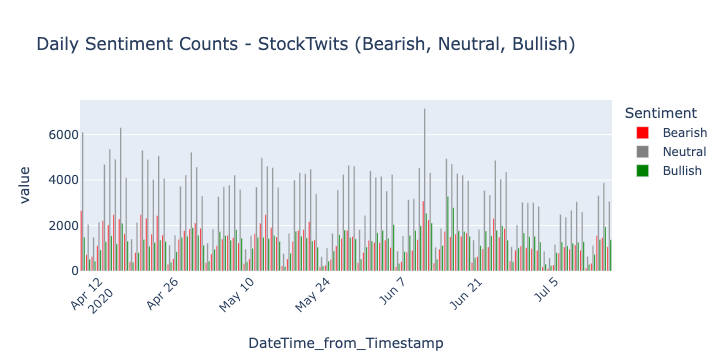
\includegraphics[width=\linewidth,height=0.6\textheight,keepaspectratio]{gfx/m4l3_notes_fig1_stocktwits_sentiment_counts.png}
\par\smallskip{\small \textbf{Hình 3.1:} Số lượng cảm xúc hàng ngày trên StockTwits (Bearish, Neutral, Bullish)}
\end{figure}

Cách tiếp cận này cho phép trực quan hóa các xu hướng cảm xúc hàng ngày trên StockTwits, với cách biểu diễn mã hóa màu rõ ràng cho các cảm xúc Bearish, Neutral và Bullish, giúp tăng khả năng diễn giải của biểu đồ. Biểu đồ cột trực quan hóa số lượng cảm xúc hàng ngày của các tin nhắn StockTwits về SPY ETF, được phân loại là Bearish (đỏ), Neutral (xám) hoặc Bullish (xanh lá). Trục hoành biểu diễn các ngày, còn trục tung biểu diễn số lượng tin nhắn. Ba cột cho mỗi ngày thể hiện số lượng của từng cảm xúc. Tính tương tác của Plotly cho phép phóng to, di chuột để xem chi tiết và khả năng chọn dữ liệu, cho phép khảo sát sâu các xu hướng cảm xúc theo thời gian.

\subsection{Phát hiện mã cổ phiếu trong dữ liệu StockTwits}

Các tin nhắn StockTwits thường chứa các mã cổ phiếu, còn được gọi là ticker hoặc cashtag. Người dùng thường đưa chúng vào để chỉ các cổ phiếu cụ thể mà họ đang thảo luận. Các mã này thường được biểu diễn bằng dấu đô la theo sau là mã chứng khoán của cổ phiếu (ví dụ \$AAPL cho Apple, \$SPY cho SPDR S\&P 500 ETF Trust).

Tương tự cách ta đã làm với tập dữ liệu Twitter, ở đây ta cũng có thể trích xuất các mã cổ phiếu từ các tin nhắn StockTwits. Đoạn mã dưới đây nhằm trích xuất các mã cổ phiếu (ticker) từ cột 'Sentence' của DataFrame \texttt{filtered\_stocktwits\_df}, đếm số lần xuất hiện của chúng và hiển thị 10 ticker được đề cập thường xuyên nhất:

\begin{lstlisting}[language=Python,escapeinside={(*@}{@*)}]
# (*@Phát@*) (*@hiện@*) (*@mã@*) (*@cổ@*) (*@phiếu@*) trong (*@dữ@*) (*@liệu@*) StockTwits
filtered_stocktwits_df['tickers'] = filtered_stocktwits_df['Sentence'].str.findall('\$[a-zA-Z]+\.*[a-zA-Z]+')
filtered_stocktwits_df.explode(['tickers'])['tickers'].value_counts().sort_values(ascending=False).head(10)
\end{lstlisting}

\begin{lstlisting}[escapeinside={(*@}{@*)}]
tickers
$SPY     553357
$QQQ      27869
$spy      12975
$SPX      11136
$AAPL     10631
$DJIA      8977
$DIA       8949
$ES        8062
$TSLA      7627
$BA        5368
Name: count, dtype: int64
\end{lstlisting}

Bảng này cho thấy 10 mã cổ phiếu (ticker) được đề cập thường xuyên nhất trong tập dữ liệu StockTwits, cùng với số lần xuất hiện tương ứng. Quan sát nổi bật nhất là sự thống trị của SPY: ticker \$SPY (SPDR S\&P 500 ETF Trust) và \$spy (phiên bản chữ thường của nó) là mã cổ phiếu được đề cập nhiều nhất với khoảng cách rất xa trong tập dữ liệu, xuất hiện hơn 553.000 lần. Điều này không đáng ngạc nhiên khi toàn bộ tập dữ liệu StockTwits này xoay quanh SPY.

Bảng cho thấy tập dữ liệu StockTwits chủ yếu tập trung vào các thảo luận về chỉ số S\&P 500 và các ETF liên quan. Tuy nhiên, cũng có sự quan tâm đáng kể đến các chỉ số thị trường lớn khác, các cổ phiếu riêng lẻ (đặc biệt là các công ty vốn hóa lớn) và các hợp đồng tương lai. Thông tin này cung cấp hiểu biết về các chủ đề và xu hướng phổ biến nhất trong cộng đồng StockTwits trong giai đoạn được phân tích.

\subsection{So sánh dữ liệu Twitter và StockTwits}

Bây giờ hãy so sánh dữ liệu Twitter và StockTwits. Đoạn mã dưới đây nhằm thực hiện việc này bằng cách tạo một biểu đồ đường. Trước hết ta tính số lượng tweet hàng ngày từ DataFrame \texttt{filtered\_twitter\_df} bằng cách nhóm dữ liệu theo phần ngày của cột 'created\_at' (dùng \texttt{dt.date} để trích xuất ngày) rồi đếm số tweet trong mỗi nhóm bằng cách đếm các giá trị không rỗng trong cột 'tweet\_text'. Ta thực hiện thao tác tương tự với DataFrame \texttt{filtered\_stocktwits\_df}, dùng cột 'DateTime\_from\_Timestamp' để nhóm theo ngày và cột 'Sentence' để đếm tin nhắn. Sau đó ta tạo và tùy chỉnh biểu đồ:

\begin{lstlisting}[language=Python,escapeinside={(*@}{@*)}]
# (*@Nhóm@*) (*@dữ@*) (*@liệu@*) Twitter theo (*@ngày@*) (*@và@*) (*@đếm@*) tweet
daily_tweet_counts_twitter = filtered_twitter_df.groupby(filtered_twitter_df['created_at'].dt.date)['tweet_text'].count()

# (*@Nhóm@*) (*@dữ@*) (*@liệu@*) StockTwits theo (*@ngày@*) (*@và@*) (*@đếm@*) tin (*@nhắn@*)
daily_tweet_counts_stocktwits = filtered_stocktwits_df.groupby(filtered_stocktwits_df['DateTime_from_Timestamp'].dt.date)['Sentence'].count()

# # (*@Tạo@*) (*@một@*) (*@hình@*) (*@và@*) (*@vẽ@*) (*@dữ@*) (*@liệu@*) Twitter (*@và@*) StockTwits
plt.figure(figsize=(12, 6))
plt.plot(daily_tweet_counts_twitter.index, daily_tweet_counts_twitter.values, label='Twitter', marker='o')
plt.plot(daily_tweet_counts_stocktwits.index, daily_tweet_counts_stocktwits.values, label='StockTwits', marker='x')

# (*@Tùy@*) (*@chỉnh@*) (*@biểu@*) (*@đồ@*)
plt.xlabel('Date')
plt.ylabel('Number of Tweets')
plt.title('Daily Tweet Counts - Twitter vs. StockTwits')
plt.legend()
plt.grid(True)

# Xoay (*@nhãn@*) (*@trục@*) x (*@để@*) (*@dễ@*) (*@đọc@*) (*@hơn@*)
plt.xticks(rotation=45, ha='right')

# (*@Điều@*) (*@chỉnh@*) (*@bố@*) (*@cục@*) (*@để@*) (*@tránh@*) (*@nhãn@*) (*@chồng@*) (*@chéo@*) (*@và@*) (*@hiển@*) (*@thị@*) (*@biểu@*) (*@đồ@*)
plt.tight_layout()
plt.show()
\end{lstlisting}

\begin{figure}[H]
\centering
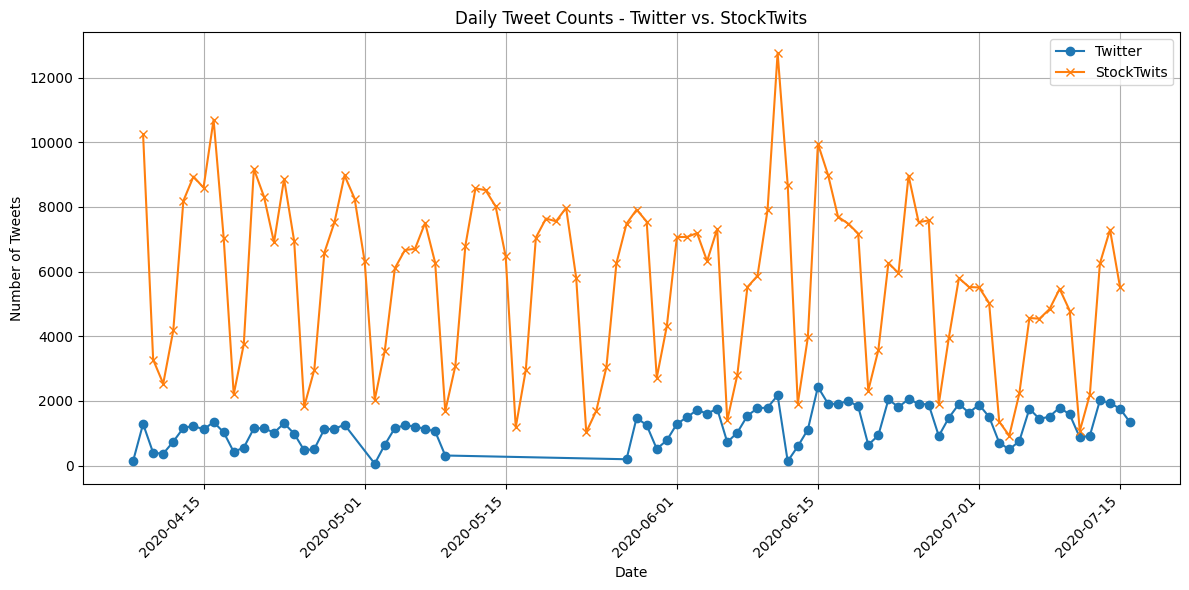
\includegraphics[width=\linewidth,height=0.6\textheight,keepaspectratio]{gfx/m4l3_notes_fig2_twitter_vs_stocktwits_daily_counts.png}
\par\smallskip{\small \textbf{Hình 3.2:} Số lượng tweet hàng ngày, Twitter so với StockTwits}
\end{figure}

Trước hết hãy quan sát rằng, trong cùng một giai đoạn, \texttt{filtered\_twitter\_df} có 99.246 hàng, trong khi \texttt{filtered\_stocktwits\_df} có 564.588 hàng. Thông tin này cung cấp ngữ cảnh có giá trị để diễn giải các biểu đồ số lượng tweet hàng ngày. Nó làm nổi bật sự khác biệt đáng kể về khối lượng dữ liệu giữa hai nền tảng trong giai đoạn đã chọn. Dưới đây là một số điểm bổ sung cần lưu ý:

\begin{itemize}
  \item Hoạt động của nền tảng: Sự khác biệt về số hàng cho thấy StockTwits có thể có hoạt động hoặc mức độ tương tác của người dùng cao hơn nhiều so với Twitter trong giai đoạn và tiêu chí lọc đã cho. Điều này có thể do nhiều yếu tố, bao gồm cơ sở người dùng, trọng tâm và mức độ phổ biến của các nền tảng trong cộng đồng đầu tư.
  \item Thu thập dữ liệu và tính toàn vẹn: Sự khác biệt về khối lượng dữ liệu có thể chịu ảnh hưởng của các phương pháp thu thập dữ liệu được sử dụng. Những người thu thập dữ liệu dùng các API hoặc nguồn dữ liệu khác nhau cho Twitter và StockTwits, và có thể có những khác biệt trong cách dữ liệu được thu thập, lọc hoặc xử lý, dẫn đến khác biệt về số hàng cuối cùng. Chúng ta cũng cần bảo đảm rằng các quy trình thu thập và lọc dữ liệu nhất quán và đáng tin cậy cho cả hai nền tảng để giảm thiểu các thiên lệch hoặc sai sót tiềm ẩn trong phân tích.
  \item Hàm ý cho phân tích: Khi so sánh các xu hướng hoặc mẫu hình giữa Twitter và StockTwits, cần lưu ý rằng số lượng tweet tuyệt đối có thể không so sánh trực tiếp được do khác biệt về khối lượng dữ liệu. Chúng ta cần cân nhắc dùng chuẩn hóa hoặc các thước đo tương đối để có những so sánh có ý nghĩa hơn.
  \item Ngữ cảnh của khoảng trống dữ liệu: Dù khoảng trống trong dữ liệu Twitter từ ngày 10 tháng 5 đến ngày 27 tháng 5 năm 2020 là điều quan trọng cần ghi nhận, cũng thiết yếu phải xem xét nó trong ngữ cảnh của tổng khối lượng dữ liệu. Nếu khoảng trống chiếm một tỷ lệ nhỏ trong tổng dữ liệu Twitter, tác động của nó lên phân tích tổng thể có thể hạn chế. Tuy nhiên, nếu khoảng trống là đáng kể so với tổng dữ liệu, nó có thể ảnh hưởng đến việc diễn giải các xu hướng hoặc mẫu hình.
\end{itemize}

Bằng cách xem xét sự khác biệt về tổng khối lượng dữ liệu và những hàm ý tiềm ẩn của nó, chúng ta có thể đưa ra các diễn giải có căn cứ hơn về các biểu đồ số lượng tweet hàng ngày và rút ra những kết luận vững chắc hơn từ phân tích. Chúng ta cần nhớ truyền đạt rõ ràng sự khác biệt về khối lượng dữ liệu cùng mọi phép chuẩn hóa hoặc điều chỉnh tỷ lệ đã áp dụng trong các báo cáo hoặc bài thuyết trình để bảo đảm tính minh bạch.

\section{Kết luận}

Trong bài học này, chúng ta đã khám phá các ứng dụng của dữ liệu thay thế. Dữ liệu thay thế trong tài chính là những nguồn dữ liệu phi truyền thống được dùng để thu được hiểu biết về xu hướng thị trường, định giá tài sản và các quyết định đầu tư. Điều này đối lập với dữ liệu truyền thống như báo cáo tài chính, hồ sơ công bố của công ty và giá thị trường. Dữ liệu văn bản từ mạng xã hội thuộc nhóm này vì nó phản ánh cảm xúc của công chúng, các bàn tán trên thị trường và sự lan truyền tin tức, những yếu tố có thể ảnh hưởng đến giá tài sản. Cụ thể, dữ liệu Twitter và StockTwits được xem là những nguồn dữ liệu thay thế có giá trị trong kỹ thuật tài chính nhờ tính thời gian thực và trọng tâm vào các thảo luận tài chính và hoạt động của thị trường chứng khoán.

Trong bài học này, chúng ta đã khám phá và so sánh dữ liệu Twitter và StockTwits để xem chúng có thể được dùng như thế nào cho phân tích tài chính. Trọng tâm chính là SPY ETF (SPDR S\&P 500 ETF Trust) và một khoảng thời gian cụ thể. Việc này bao gồm lấy dữ liệu từ cả Twitter và StockTwits, điều chỉnh múi giờ và xử lý retweet trên Twitter; tạo các biểu đồ để xem có bao nhiêu tweet được đăng mỗi ngày trên từng nền tảng nhằm hiểu sự khác biệt về khối lượng dữ liệu và hoạt động của người dùng.

\textbf{Tài liệu tham khảo}

\begin{itemize}
  \item Bruno Taborda, Ana de Almeida, José Carlos Dias, Fernando Batista, Ricardo Ribeiro, April 15, 2021, ``Stock Market Tweets Data'', IEEE Dataport, doi: \url{https://dx.doi.org/10.21227/g8vy-5w61}
  \item Liu, Jin-Xian (2022). SPY\_stocktwits\_messages.csv. figshare. Dataset. \url{https://doi.org/10.6084/m9.figshare.20237736.v1}
\end{itemize}
